
%(BEGIN_QUESTION)
% Copyright 2011, Tony R. Kuphaldt, released under the Creative Commons Attribution License (v 1.0)
% This means you may do almost anything with this work of mine, so long as you give me proper credit

This Siemens S7-200 PLC has been programmed to count the number of people in a room, by incrementing a counter every time a person enters through the doorway, and decrementing that same counter whenever someone exits through the same doorway.  The two optical switches activate whenever their respective light beams are broken by someone passing through.  Their horizontal separation is just a couple of inches -- much less than the girth of a person's torso.  The operating status of each switch is that it energizes the PLC input when the light beam is broken:

$$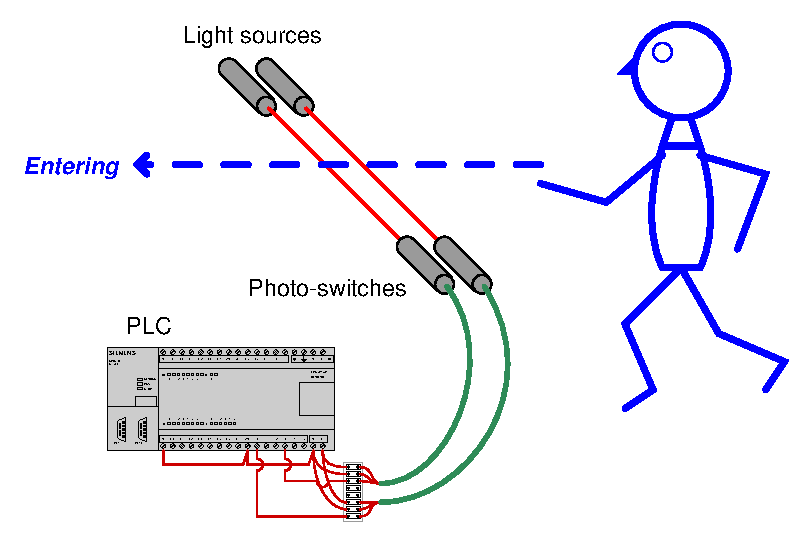
\includegraphics[width=15.5cm]{i00185x01.eps}$$

Examine the program in this PLC for counting people, and determine how it is able to differentiate between a person entering the room and a person leaving the room:

$$\includegraphics[width=15.5cm]{i00185x02.eps}$$

\vskip 20pt \vbox{\hrule \hbox{\strut \vrule{} {\bf Suggestions for Socratic discussion} \vrule} \hrule}

\begin{itemize}
\item{} Explain how a {\it timing diagram} of the switch states would be helpful in analyzing the operation of this PLC program.
\item{} {\it Transition} (edge-detecting) functions are implemented in Allen-Bradley PLCs using the {\it one-shot rising} (OSR) instruction.  Research how the OSR instruction is used, and how it differs from the ``P'' and ``N'' contacts shown in this Siemens PLC program.
\item{} Will this system still function properly if the optical sensors are spaced farther apart than the width of a human body?  Explain why or why not.
\end{itemize}

\underbar{file i00185}
%(END_QUESTION)





%(BEGIN_ANSWER)

Hint: the ``P'' contact instructions are {\it positive transition} instructions, ``activating'' whenever their respective bits transition from 0 to 1, but returning to an ``inactive'' state whenever the bit value holds at either 0 or 1.

%(END_ANSWER)





%(BEGIN_NOTES)

This counter instruction increments if ever input {\tt I1.3} transitions from low to high as input {\tt I1.0} is already high (i.e. the exact moment the left-hand beam breaks when the right-hand beam has already been broken -- the person is moving from right to left).

\vskip 10pt

The counter decrements if ever input {\tt I1.0} transitions from low to high as input {\tt I1.3} is already high (i.e. the exact moment the right-hand beam breaks when the left-hand beam has already been broken -- the person is moving from left to right).

%INDEX% PLC, ladder logic program analysis and explanation (Siemens S7-200)

%(END_NOTES)


